%%%%%%%%%%%%%%%%%%%%%%%%%%%%%%%%%%%%%%%%%%%%%%%%%%%%%%%%%%%%%%%%%%%%%%%%%%%%%%%%
\section{Considerações iniciais}

Sistemas de reconhecimento de imagens comumente utilizam uma imagem em níveis de cinza ($2^3 = 8$ bits, $2^8 = 256$ intensidades) para as etapas subsequentes à extração de características. Dá-se o nome de quantização à etapa responsável por esta redução do nível de intensidades de uma imagem. Ao aplicar a quantização na etapa de pré-processamento, é esperada a redução da complexidade do vetor de características logo no início do processo, beneficiando todos os passos subsequentes.

Com o objetivo de analisar o impacto do uso da quantização, foram utilizados diferentes parâmetros de quantização, combinados com quatro métodos de extração de cor e um de textura. Esses métodos foram escolhidos de acordo com os resultados apresentados por \citeonline{Penatti2012} e \citeonline{Wang2009}. Este capítulo aborda a quantização de imagens antes da etapa de extração de características, assim como os métodos utilizados para tal, já apresentados na Seção~\ref{sec:quantizacao}. Após, apresenta os resultados encontrados ao aplicar os métodos de quantização de imagens no \textit{pipeline} de reconhecimento. Para cada experimento realizado são descritos: a base de imagens; o protocolo utilizado; os resultados encontrados e a sua relevância. Os resultados devem refletir melhoras nas etapas subsequentes, como uma melhor acurácia na etapa de classificação ou a redução do tempo de processamento.


%%%%%%%%%%%%%%%%%%%%%%%%%%%%%%%%%%%%%%%%%%%%%%%%%%%%%%%%%%%%%%%%%%%%%%%%%%%%%%%%
\section{Quantização de imagens}

O \textit{pipeline}  de reconhecimento de imagens comumente envolve um passo de conversão de imagens coloridas em imagens com apenas um canal de cor. Obtém-se, assim, uma imagem quantizada, que pode ser então processada por métodos de extração de características. Dessa forma, cada imagem --- originalmente no espaço de cor RGB --- é convertida a um único canal com $C$ níveis de intensidade. Após, são utilizados os métodos de extração de características para obter um vetor representativo da imagem. A Figura \ref{fig:quant:quantizationFlow} ilustra esses passos, desde a aquisição até a classificação das imagens.

\begin{figure}[!htbp]
  \begin{center}
    \centering
    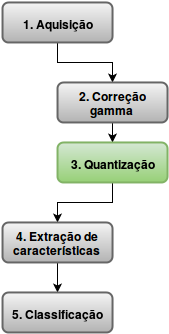
\includegraphics[width=0.25\linewidth]{\detokenize{figuras/quantizacao/quantizationFlow.png}}
  \end{center}
  \caption[O pipeline de reconhecimento de imagens pode envolver uma etapa de conversão de imagens coloridas em imagens em escala de cinza, obtendo uma imagem quantizada que pode ser então processada por métodos de extração de características. O vetor com essas características é então dado como entrada a algum método de classificação.]{O pipeline de reconhecimento de imagens pode envolver uma etapa de conversão imagens coloridas em imagens em escala de cinza, obtendo uma imagem quantizada que pode ser então processada por métodos de extração de características. O vetor com essas características é então dado como entrada a um método posterior de classificação. \\ \textit{Fonte:~Elaborado pela autora.}}
  \label{fig:quant:quantizationFlow}
\end{figure}

Cada método de quantização se comporta diferentemente para uma dada imagem RGB. O método \emph{Intensidade} (Equação \ref{eq:intensidade}), por exemplo, mapeia todas as permutações dos mesmos valores de RGB para a mesma cor de cinza. Dessa forma, produz um plano no espaço RGB conforme mostrado na Figura \ref{fig:quant:plano}. O efeito do método \emph{Gleam} (Equação \ref{eq:gleam}) é similar, mas dada a natureza da função \textit{gamma} (i.e. transformação não linear que define a relação entre o valor do pixel e sua real luminância), cobre uma superfície curva. Tal resultado também é alcançado utilizando o método \emph{Intensidade'} (método \emph{Intensidade} corrigido por \textit{gamma}). Independente do método utilizado, o resultado é o mapeamento de características cromáticas bem diferentes em valores de intensidades similares. Ou seja, intensidades distintas podem ser convertidas em intensidades próximas, podendo aumentar a confusão entre objetos. Pode-se imaginar esse efeito em uma imagem natural que retrata céu e grama. Considere a confusão das intensidades resultantes da região de céu e grama (e.g RGB(0, 0, 255) e RGB(0, 255, 0), respectivamente): apesar de terem intensidades bem distintas em RGB, os valores em apenas um canal de cor podem estar relativamente próximos. Os métodos\emph{Luminância'} (Equação \ref{eq:luminancia}) e \emph{Luma} (Equação \ref{eq:luma}) procuram aprimorar essa quantização ao ponderar a combinação linear dos canais. Esses métodos são normalmente considerados melhores por se aproximarem ao modelo visual humano, que pondera as intensidades através do número de cones sensíveis às cores vermelho, verde e azul. O método MSB também tenta enfatizar as diferenças cromáticas, ao ordenar os bits de cores em um único canal. Para mais detalhes sobre esses métodos, consulte Seção \ref{sec:quantizacao}.

\begin{figure}[!htbp]
  \begin{center}
    \centering
    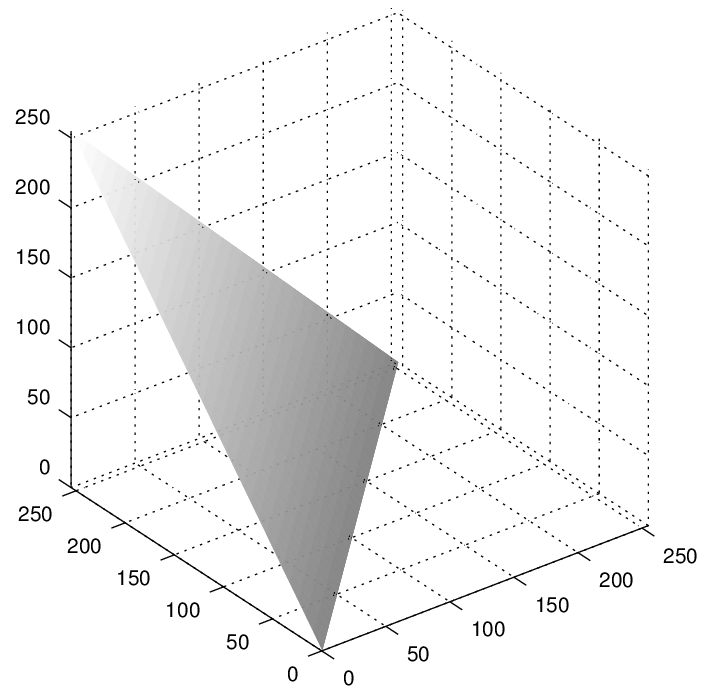
\includegraphics[width=0.5\linewidth]{\detokenize{figuras/quantizacao/plano.png}}
  \end{center}
  \caption[Plano no espaço RGB, computado pelo método de conversão para escala de cinza \emph{Intensidade}, quando um dos canais de cor (vermelho, verde ou azul) possui valor 255. O resultado é o mapeamento de características cromáticas bem diferentes em valores de intensidade similares.]{Plano no espaço RGB, computado pelo método de conversão para escala de cinza \emph{Intensidade}, quando um dos canais de cor (vermelho, verde ou azul) possui valor 255. O resultado é o mapeamento de características cromáticas bem diferentes em valores de intensidade similares. \\ \textit{Fonte:~\citeonline{Ponti2016}.}}
  \label{fig:quant:plano}
\end{figure}

Exemplos de imagens obtidas após os métodos de quantização apresentados anteriormente podem ser vistos na Figura \ref{fig:quant:quantizacoes}. A barra de gradientes abaixo da imagem dos pincéis demonstra como os métodos de quantização se comportam dada a variação das intensidades. É possível notar que os métodos \emph{Luminância'} e MSB conseguiram melhor discriminar as cores. Além disso, o mapa de cores MSB obteve um maior número de intensidades únicas, quando comparado aos demais métodos.

\begin{figure}[!htbp]
  \begin{center}
    \subfloat[Original]{
      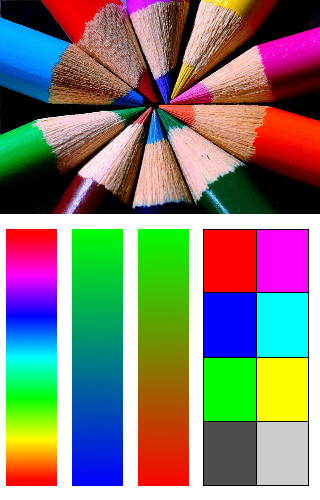
\includegraphics[width=.18\linewidth]{\detokenize{figuras/quantizacao/fig_quanttest.png}}
      \label{fig:quant:original}
    }
    \subfloat[\emph{Gleam}]{
      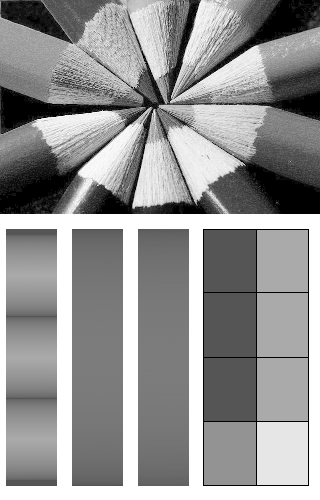
\includegraphics[width=.18\linewidth]{\detokenize{figuras/quantizacao/fig_quantGleam.png}}
    }
    \subfloat[\emph{Intensidade'}]{
      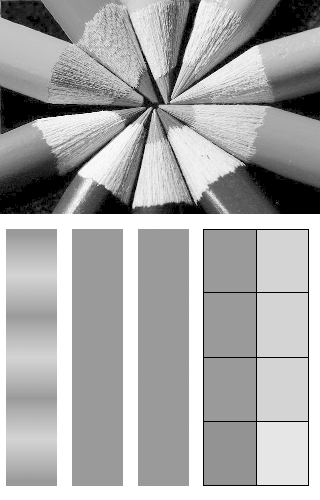
\includegraphics[width=.18\linewidth]{\detokenize{figuras/quantizacao/fig_quantIntensity.png}}
    }
    \subfloat[\emph{Luminância'}]{
      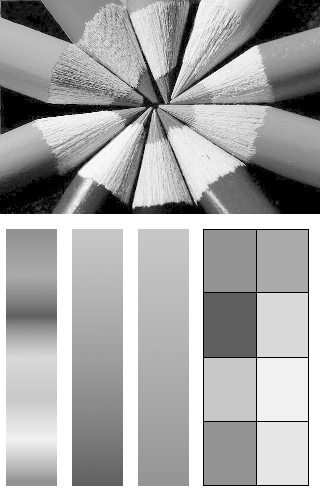
\includegraphics[width=.18\linewidth]{\detokenize{figuras/quantizacao/fig_quantLuminance.png}}
    }
    \subfloat[MSB]{
      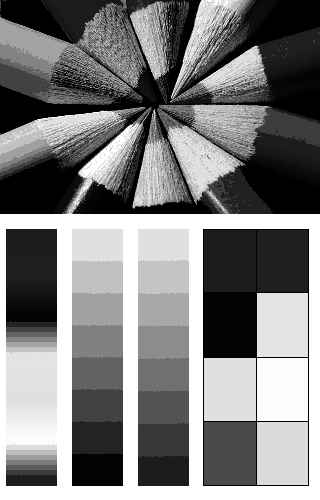
\includegraphics[width=.18\linewidth]{\detokenize{figuras/quantizacao/fig_quantMSB.png}}
    }
    \hspace{0.1\textwidth}
  \end{center}
  \caption[Resultado da aplicação de métodos de quantização. A imagem original \protect\subref{fig:quant:original} resultou em versões de um canal de cor com 232 intensidades únicas para o método (e) MSB e 184 intensidades para os demais métodos. Ao analisar-se as barras de gradiente, assim como as paletas de cores, observa-se que os métodos\emph{Luminância'} e MSB conseguiram uma melhor discriminação entre intensidades.]{Resultado da aplicação de métodos de quantização. A imagem original \protect\subref{fig:quant:original} resultou em versões de um canal de cor com 232 intensidades únicas para o método (e) MSB e 184 intensidades para os demais métodos. Ao analisar-se as barras de gradiente, assim como as paletas de cores, observa-se que os métodos\emph{Luminância'} e MSB conseguiram uma melhor discriminação entre intensidades. \\ \textit{Fonte:~\citeonline{Ponti2016}.}}
  \label{fig:quant:quantizacoes}
\end{figure}

% A Tabela \ref{tab:quantizacao} apresenta alguns exemplos numéricos, com a saída de cada método. Nesse caso, as entradas são tuplas de valores $(R, G, B)$. Note que a correção \textit{gamma} deve ser computada em um intervalo de valores reais $0-1$, que depois é mapeado para o intervalo $0-255$.

Complementando, a Figura \ref{fig:quant:avioes} apresenta um exemplo de redução de cores utilizando o método MSB para um par de imagens da base de dados \emph{Caltech101-600}~\cite{Fei-Fei2007}. É possível notar que há uma certa preservação das cores, especialmente quando utilizados entre 64 e 256 níveis. Com apenas 32 intensidades, as imagens ainda lembram a sua versão original, mas há perda considerável de informação, principalmente em regiões da imagem com pouco contraste.

\begin{figure}[!htbp]
  \begin{center}
    \centering
    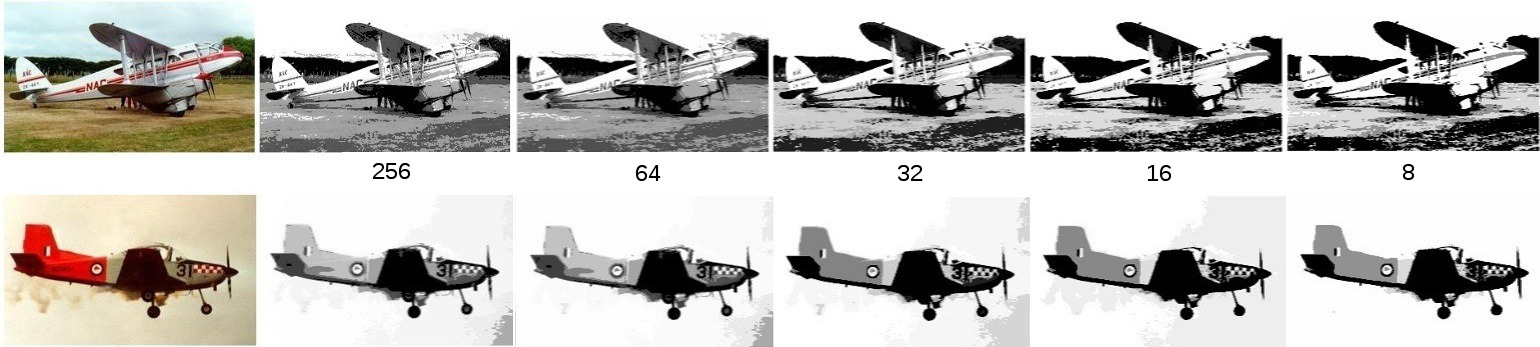
\includegraphics[width=\linewidth]{\detokenize{figuras/quantizacao/fig_quantizationexample.jpg}}
  \end{center}
  \caption[Exemplo de duas imagens da base de dados \emph{Caltech101-600} com variações no parâmetro de cor utilizando o método MSB. Da esquerda para a direita: imagem original 24-bits e suas versões quantizadas com: 256, 64, 32, 16 e 8 intensidades.]{Exemplo de duas imagens da base de dados \emph{Caltech101-600} com variações no parâmetro de cor utilizando o método MSB. Da esquerda para a direita: imagem original 24-bits e suas versões quantizadas com: 256, 64, 32, 16 e 8 intensidades. \\ \textit{Fonte:~\citeonline{Ponti2016}.}}
  \label{fig:quant:avioes}
\end{figure}

%%%%%%%%%%%%%%%%%%%%%%%%%%%%%%%%%%%%%%%%%%%%%%%%%%%%%%%%%%%%%%%%%%%%%%%%%%%%%%%%
\section{Experimentos}
\label{sec:resultados-quantizacao}

O objetivo desta seção é mostrar os efeitos da etapa de quantização e como ela pode ser utilizada para reduzir a dimensionalidade do espaço de características ou a complexidade em etapas posteriores do \textit{pipeline} de classificação. A Figura~\ref{fig:quant:flowResult} demonstra o fluxo das operações, juntamente com os métodos utilizados nos experimentos. Inicialmente, as imagens foram quantizadas em 256, 128, 64, 32 e 16 intensidades. Dependendo do método de conversão para a escala de cinza, a correção \textit{gamma} é realizada (ver Seção \ref{sec:quantizacao}). Após, suas características são extraídas e duas etapas distintas de experimentos são realizadas:

\begin{enumerate}
  \item Experimentos utilizando um método de extração de características seguido pela classificação (sem posterior seleção de características);
  \item Experimentos utilizando o vetor resultante da concatenação de todos os métodos de extração, seguido pela classificação com e sem a seleção de características.
\end{enumerate}

\begin{figure}[!htbp]
  \begin{center}
    \centering
    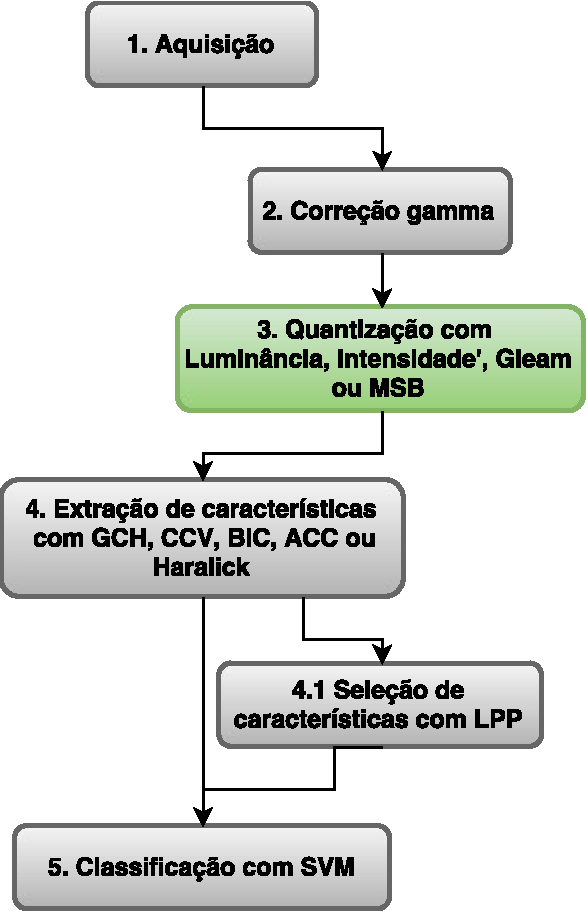
\includegraphics[width=0.4\linewidth]{\detokenize{figuras/quantizacao/quantizationResult.pdf}}
  \end{center}
  \caption[Fluxo das operações e os métodos utilizados nos experimentos. Após a aquisição da imagem, ela é convertida para escala de cinza e seus níveis de cor são reduzidos de acordo com um parâmetro da quantização (i.e.\ número de intensidades). Dependendo do método, a correção \emph{gamma} é realizada. A imagem quantizada serve então como entrada para um método de extração de características e posteriormente é classificada com \emph{SVM}. Uma das etapas de experimentos prevê também a concatenação de todos os vetores extraídos e a seleção das características com \emph{LPP} antes da classificação.]{Fluxo das operações e os métodos utilizados nos experimentos. Após a aquisição da imagem, ela é convertida para escala de cinza e seus níveis de cor são reduzidos de acordo com um parâmetro da quantização (i.e.\ número de intensidades). Dependendo do método, a correção \emph{gamma} é realizada. A imagem quantizada serve então como entrada para um método de extração de características e posteriormente é classificada com \emph{SVM}. Uma das etapas de experimentos prevê também a concatenação de todos os vetores extraídos e a seleção das características com \emph{LPP} antes da classificação. \\ \textit{Fonte:~Elaborado pela autora.}}
  \label{fig:quant:flowResult}
\end{figure}

%%%%%%%%%%%%%%%%%%%%%%%%%%%%%%%%%%%%%%%%%%%%%%%%%%%%%%%%%%%%%%%%%%%%%%%%%%%%%%%%
\subsection{Base de Imagens}

Três bases de imagens, exemplificadas na Figura~\ref{fig:quant:bases}, foram utilizadas nestes experimentos de quantização:
\begin{itemize}
\item[] \textbf{Corel-1000} \cite{Wang2001}: consiste em dez classes balanceadas de imagens naturais, com algumas classes bem definidas e algumas não;
\item[] \textbf{Caltech101-600} \cite{Fei-Fei2007}: contém fotos e desenhos. Dessa base, foi utilizado um conjunto de seis classes balanceadas: aviões, bonsais, candelabros, tartarugas, motocicletas e relógios;
\item[] \textbf{Produce-1400} \cite{Rocha2010}: também conhecido como base de vegetais e frutas tropicais. Composta por imagens com um fundo similar mas mudanças representativas na iluminação, no número de objetos e na escala. Apesar da oclusão parcial de objetos ser observada, essa classe possui dados bem comportados.
\end{itemize}

\begin{figure}[!htbp]
  \begin{center}
    \subfloat[Base de imagens Corel-1000]{
      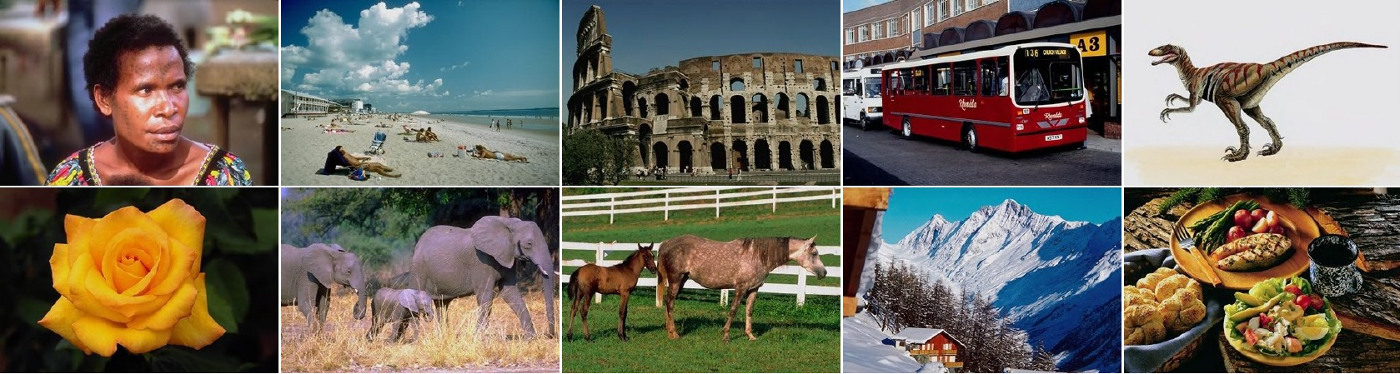
\includegraphics[width=\linewidth]{\detokenize{figuras/quantizacao/fig_COREL_dataset.jpg}}
    }
    \newline
    \subfloat[Base de imagens Caltech101-600]{
      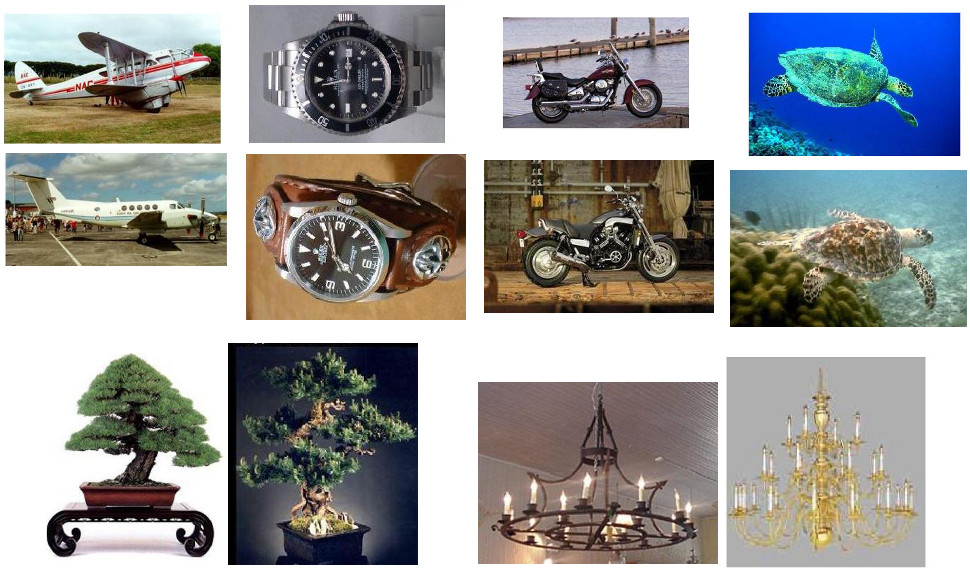
\includegraphics[width=\linewidth]{\detokenize{figuras/quantizacao/fig_Caltech101_dataset.jpg}}
    }
    \newline
    \subfloat[Base de imagens Produce-1400]{
      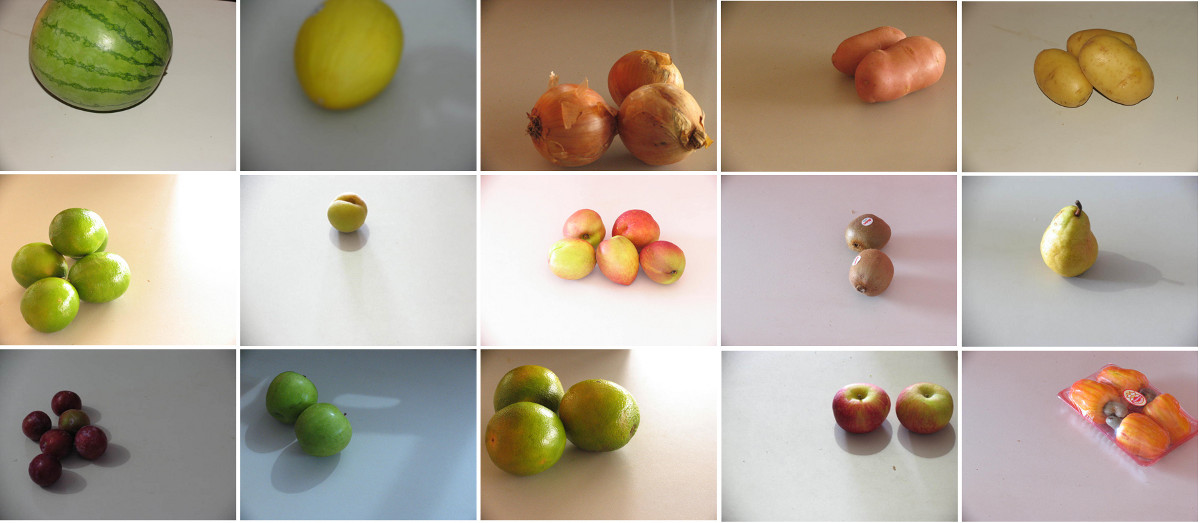
\includegraphics[width=\linewidth]{\detokenize{figuras/quantizacao/fig_Produce_dataset.jpg}}
    }
  \end{center}
  \caption[Bases de imagens Corel-1000, Caltech101-600 e Produce-1400. Elas são utilizadas nos experimentos de quantização.]{Bases de imagens Corel-1000, Caltech101-600 e Produce-1400. Elas são utilizadas nos experimentos de quantização.\\ \textit{Fonte:~\citeonline{Ponti2016}.}}
  \label{fig:quant:bases}
\end{figure}

Considerando que estes experimentos possuem foco na redução da dimensionalidade, para evitar o problema do desbalanceamento as bases Produce-1400 e Caltech101-600 foram modificadas. Dessa forma, as classes disponíveis foram balanceadas ao remover imagens das classes majoritárias.

%%%%%%%%%%%%%%%%%%%%%%%%%%%%%%%%%%%%%%%%%%%%%%%%%%%%%%%%%%%%%%%%%%%%%%%%%%%%%%%%
\subsection{Protocolo}

Os experimentos foram realizados com uma validação cruzada de \textit{10-fold}. Considerando que as bases estão balanceadas e que a seleção de exemplos para a validação cruzada é estratificada, a medida estatística de \textit{acurácia} foi utilizada para avaliar o desempenho da classificação. O seguinte protocolo foi seguido para a obtenção dos resultados:

\begin{enumerate}
\item \textbf{Quantização}: com os métodos \emph{Intensidade'}, \emph{Gleam}, \emph{Luminância'} e MSB.
\item \textbf{Extração de características}: utilizando os métodos --- e parâmetros escolhidos com base nas recomendações dos artigos que proporam tais métodos --- a seguir:
  \begin{itemize}
    \item \textit{Auto Color Correlogram} (ACC): a métrica de distância utilizada entre os pixels $p(x,y)$ e $q(s,t)$ é a tabuleiro de xadrez $D_8(p,q) = Max(|x-s| + d, |y-t| + d)$ para quatro distâncias $d =$ 1, 3, 5 e 7;
    \item \textit{Border-Interior Classification} (BIC): com uma vizinhança de quatro pixels;
    \item \textit{Color Coherence Vector} (CCV): adotando um valor de $\mathit{threshold} = 25$ para a classificação dos pixels entre coerentes e incoerentes;
    \item Haralick-6: o pixel vizinho para o qual iniciar a computar a matriz de co-ocorrência foi o pixel à direita.
  \end{itemize}
\item \textbf{Redução da dimensionalidade}: a projeção utilizando \textit{Locality Preserving Projections} (LPP) foi realizada com o parâmetro $k =$ 128, 64, 32 e 16 dimensões e 10 vizinhos. Esse parâmetro foi determinado empiricamente e não influencia consideravelmente a acurácia.
\item \textbf{Classificação}: realizada com o classificador \textit{Support Vector Machines} (SVM). Os parâmetros para essa etapa foram encontrados utilizando uma \textit{grid search} no conjunto de treinamento.
\end{enumerate}

%%%%%%%%%%%%%%%%%%%%%%%%%%%%%%%%%%%%%%%%%%%%%%%%%%%%%%%%%%%%%%%%%%%%%%%%%%%%%%%%
\section{Resultados e Discussão}

A Figura \ref{fig:quant:results} ilustra a acurácia média para o primeiro conjunto de experimentos: para cada combinação de base de dados e método de extração, são demonstrados seis resultados de acurácia correspondentes à quantização para 256, 128, 64, 32, 16 e 8 intensidades. Com base nessa figura é possível identificar que o método para obter a imagem quantizada tem um impacto significativo na acurácia da classificação. Além disso, a redução de 256 para um menor número de intensidades normalmente manteve as acurácias e em alguns casos resultou em uma ligeira melhora, especialmente para os níveis de 128 e 64.

\begin{figure}[!htbp]
  \begin{center}
    \centering
    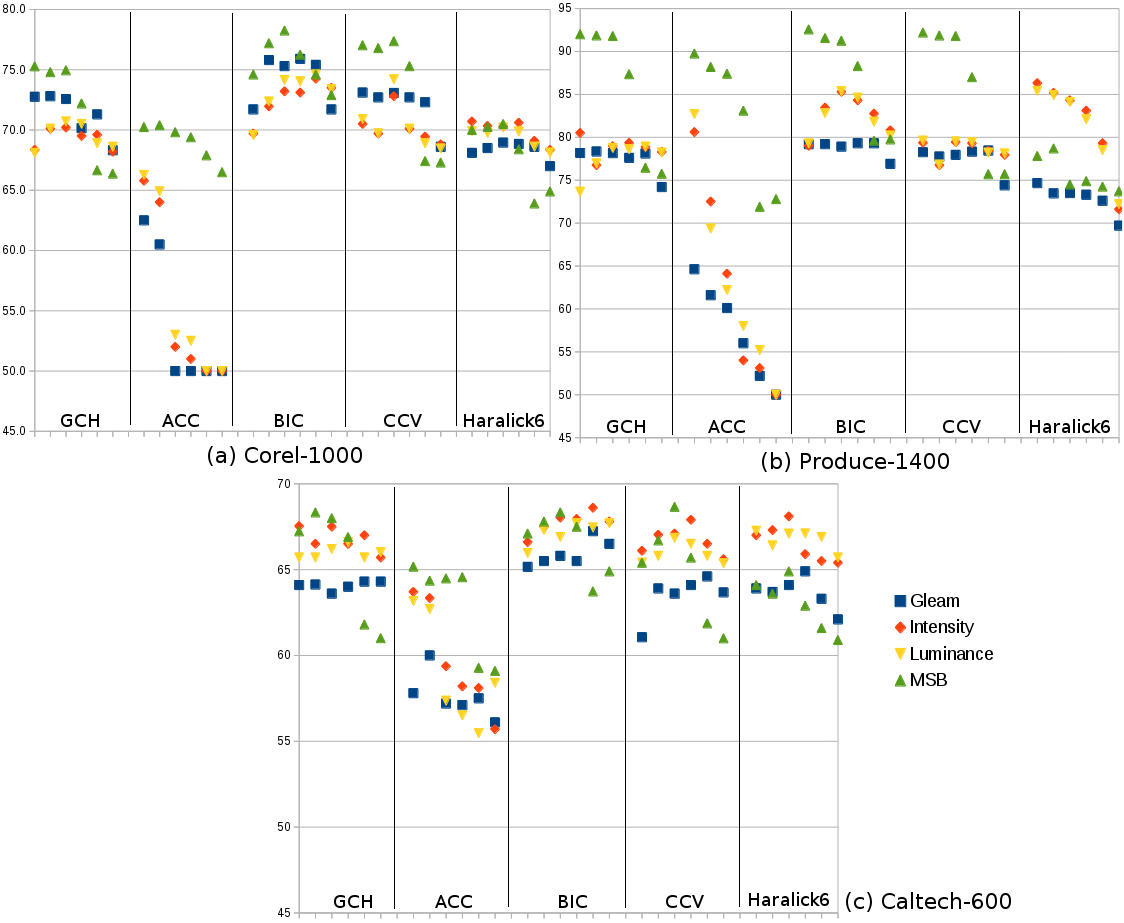
\includegraphics[width=\linewidth]{\detokenize{figuras/quantizacao/fig_results_individual.png}}
  \end{center}
  \caption[Resultados para as bases Corel-1000 (a), Produce-1400 (b) e Caltech101-600 (c), utilizando todos os métodos de quantização. Para cada método de extração de características a acurácia é resultante da sua aplicação utilizando 256, 128, 64, 32, 16 e 8 intensidades, da esquerda para a direita.]{Resultados para as bases Corel-1000 (a), Produce-1400 (b) e Caltech101-600 (c), utilizando todos os métodos de quantização. Para cada método de extração de características a acurácia é resultante da sua aplicação utilizando 256, 128, 64, 32, 16 e 8 intensidades, da esquerda para a direita. \\ \textit{Fonte:~\citeonline{Ponti2016}.}}
  \label{fig:quant:results}
\end{figure}

Considerando que a utilização de apenas 16 e 8 intensidades resultou em uma acurácia muito inferior, o restante dos resultados utilizam 256, 128, 64 e 32 intensidades. A partir dessa análise geral, uma análise mais específica foi realizada com a combinação dos métodos BIC e MSB; e Haralick e \emph{Luminância'}. O teste estatístico ANOVA foi realizado para comparar as acurácias dos experimentos das Figuras \ref{fig:quant:boxplotBIC} e \ref{fig:quant:boxplotHaralick}. Para identificar se algum método obteve uma diferença significativa no valor de acurácia, foi utilizado o teste \sigla{HSD}{\textit{Honest Significant Difference}} de Tukey. Um nível de significância de $\alpha = 0.01$ foi utilizado. Por conta disso, os \textit{boxplots} em cinza correspondem aos dados com diferença estatística relevante quando comparados com a acurácia de 256 intensidades, obtendo um $\textit{p-value} < 0.01$.

% O boxplot para 256, 128, 64 e 32 intensidades com os métodos \emph{BIC} e MSB está demonstrado na Figura \ref{fig:quant:boxplotBIC}.

De acordo com o teste estatístico representado na Figura \ref{fig:quant:boxplotBIC}, utilizar características de cor (extraídas com o método BIC) e níveis de quantização providos pelo método MSB demonstrou resultados melhores do que o \textit{baseline} de 256 intensidades para as bases Corel-1000 (128, 64 e 32 intensidades) e Caltech101-600 (64 intensidades). O único resultado que piorou significativamente foi para 32 intensidades da base de imagens Produce-1400. Portanto, converter as imagens para a escala de cinza e reduzir os 256 possíveis valores para apenas 64 provou uma boa escolha de processamento anterior a extração de características. Ou seja, $d \approx D/4$. Menores valores podem degradar os resultados em características de textura, como mostrado na Figura \ref{fig:quant:boxplotHaralick}.

\begin{figure}[!htbp]
  \begin{center}
    \centering
    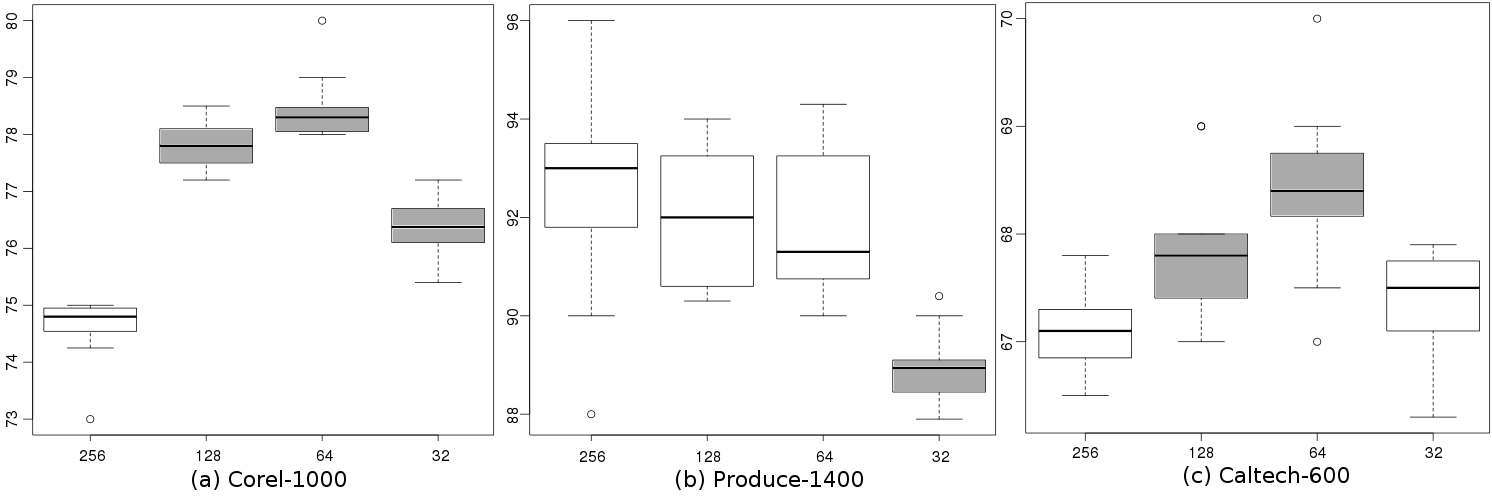
\includegraphics[width=\linewidth]{\detokenize{figuras/quantizacao/fig_results_individual_boxplotBIC.png}}
  \end{center}
  \caption[Resultados de acurácia média da classificação utilizando o método de quantização MSB considerando 256, 128, 64 e 32 intensidades com o método de extração de características BIC. Os \textit{boxplots} em cinza correspondem às significâncias estatísticas com $\textit{p-value} < 0.01$ quando comparado à acurácia de 256 intensidades.]{Resultados de acurácia média da classificação utilizando o método de quantização MSB considerando 256, 128, 64 e 32 intensidades com o método de extração de características BIC. Os  \textit{boxplots} em cinza correspondem às significâncias estatísticas com $\textit{p-value} < 0.01$ quando comparado à acurácia de 256 intensidades.\\ \textit{Fonte:~\citeonline{Ponti2016}.}}
  \label{fig:quant:boxplotBIC}
\end{figure}

\begin{figure}[!htbp]
  \begin{center}
    \centering
    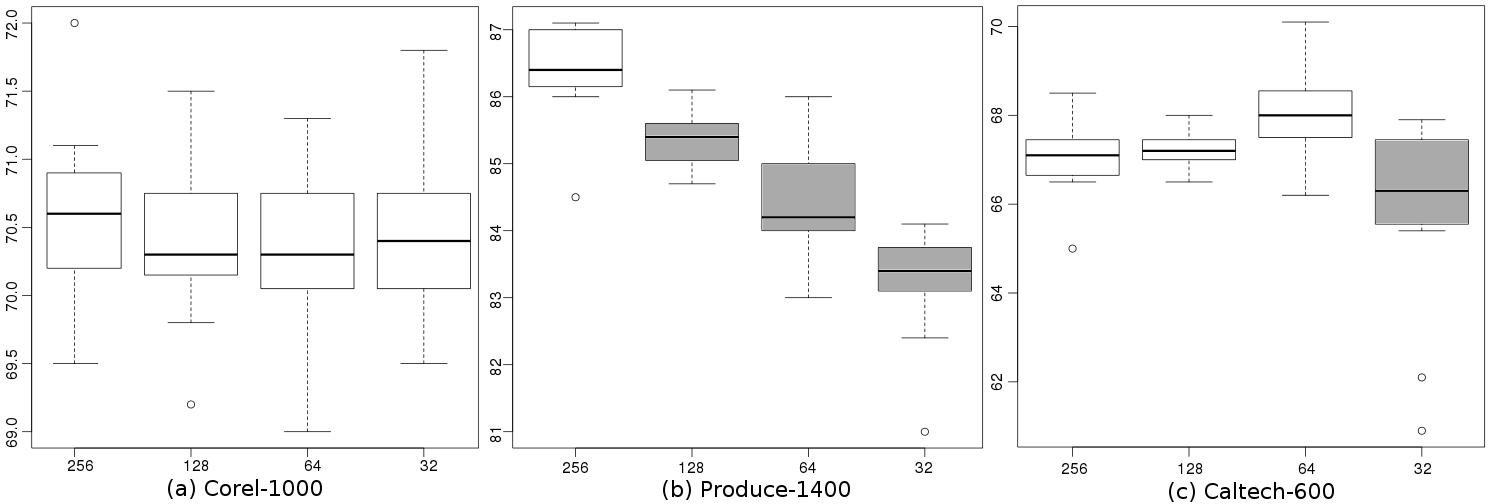
\includegraphics[width=\linewidth]{\detokenize{figuras/quantizacao/fig_results_individual_boxplotHaralick.png}}
  \end{center}
  \caption[Acurácia média da classificação após a utilização do método de quantização \emph{Luminância'} considerando 256, 128, 64 e 32 intensidades com o descritor Haralick. Os  \textit{boxplots} em cinza correspondem às significâncias estatísticas com $\textit{p-value} < 0.01$ quando comparado à acurácia de 256 intensidades.]{Acurácia média da classificação após a utilização do método de quantização \emph{Luminância'} considerando 256, 128, 64 e 32 intensidades com o descritor Haralick. Os \textit{boxplots} em cinza correspondem às significâncias estatísticas com $\textit{p-value} < 0.01$ quando comparado à acurácia de 256 intensidades. \\ \textit{Fonte:~\citeonline{Ponti2016}.}}
  \label{fig:quant:boxplotHaralick}
\end{figure}

Uma outra comparação importante é entre a redução de dimensionalidade obtida com métodos de quantização versus o método LPP. A redução de dimensionalidade obtida com os métodos MSB, BIC e LPP está ilustrada na Figura \ref{fig:quant:boxplotMSBLPP}. A imagem de entrada foi convertida para escala de cinza com o método MSB em 256 intensidades. Essa imagem foi dada como entrada para o método de extração de características BIC, que resultou em um vetor dado como entrada para o LPP. Esse último passo teve o objetivo de produzir versões reduzidas desse vetor para 256, 128 e 64 dimensões. As acurácias obtidas foram então comparadas com a classificação dos vetores reduzidos apenas pela quantização. Como a comparação foi feita em pares, foram realizados testes $t$ de Student sobre a suposição de dois exemplos independentes com variâncias desiguais e um nível de significância de $0.01$. O método de quantização obteve valores de acurácia menores à utilização do LPP em três experimentos: 256 intensidades com a base Corel-1000 e com 256 e 64 na base Produce-1400. Para a base Caltech101-600 a quantização foi melhor com 256 e 128 dimensões. O restante dos experimentos não apresentaram diferença estatística relevante. Apesar da perda de acurácia em alguns casos, é importante notar que --- se utilizado um número de intensidades correto --- é possível manter ou até mesmo melhorar as acurácias após a redução da dimensionalidade. Isso pode ser observado na Figura \ref{fig:quant:boxplotMSBLPP} referente à base de dados Caltech101-600.

\begin{figure}[!htbp]
  \begin{center}
    \centering
    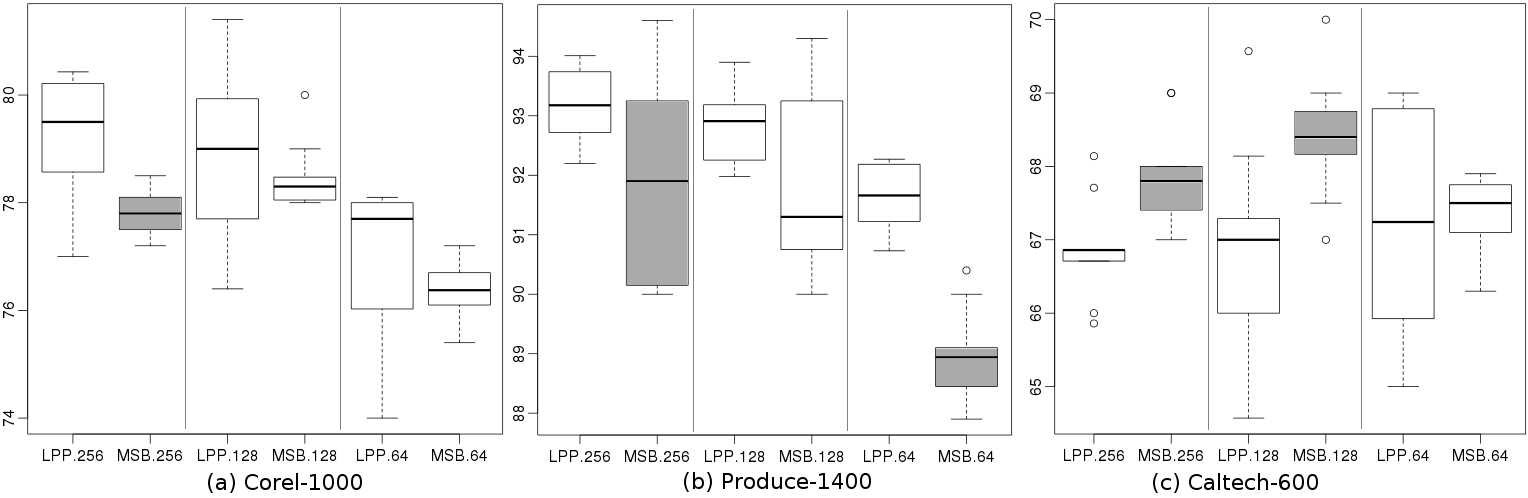
\includegraphics[width=\linewidth]{\detokenize{figuras/quantizacao/fig_results_individual_boxplotMSBLPP.png}}
  \end{center}
  \caption[Resultados de acurácia para os método MSB (quantização), LPP (redução de dimensionalidade) e BIC (extração de características). A comparação do LPP versus MSB foi realizada com a mesma dimensionalidade. Os boxplots em cinza correspondem às significâncias estatísticas com $p < 0.01$ quando comparado a acurácia de 256 intensidades.]{Resultados de acurácia para os método MSB (quantização), LPP (redução de dimensionalidade) e BIC (extração de características). A comparação do LPP versus MSB foi realizada com a mesma dimensionalidade. Os boxplots em cinza correspondem às significâncias estatísticas com $p < 0.01$ quando comparado a acurácia de 256 intensidades. \\ \textit{Fonte:~\citeonline{Ponti2016}.}}
  \label{fig:quant:boxplotMSBLPP}
\end{figure}

O número de dimensões de um vetor resultante de apenas um método de extração de características pode ser considerado baixo. É comum a extração de diversos descritores para uma determinada situação, considerando que normalmente não é claro qual método deveria ser utilizado em cada caso. Por conta disso, os próximos experimentos foram realizados a partir da concatenação de tais características. O objetivo destes experimentos é verificar se a concatenação de todos os descritores pode melhorar os resultados de acurácia. Além disso, comparar os resultados com os experimentos anteriores, afim de verificar se a quantização pode ser uma alternativa à redução da dimensionalidade com métodos convencionais (LPP, neste caso). A melhor configuração encontrada com os experimentos anteriores, entre tamanho do vetor e acurácia, foi utilizando 128 e 64 intensidades.

A redução do número de intensidades influencia a dimensionalidade original $D$. O número de características em relação ao número de intensidades, concatenando todos os vetores resultantes dos métodos de extração de características, é: 256 intensidades --- 2310 características; 128 intensidades --- 1160 características; 64 intensidades --- 582 características; 32 intensidades --- 294 características; e 16 intensidades --- 150 características.

Primeiramente, as imagens foram convertidas para escala de cinza e mantidas com 256 intensidades. Essas imagens foram descritas por todos os métodos de extração e suas características concatenadas em um vetor com dimensão original $D=2310$. A redução de dimensionalidade com LPP foi realizada para $d$ = 1160, 582, 294 e 150. Ou seja, produzindo vetores com o mesmo tamanho dos obtidos apenas com a quantização como método de redução da dimensionalidade. A Figura \ref{fig:quant:resultsFull} mostra os resultados utilizando LPP para as três bases de imagens. Note que o método de quantização MSB resultou em acurácias melhores que os outros métodos.

\begin{figure}[!htbp]
  \begin{center}
    \centering
    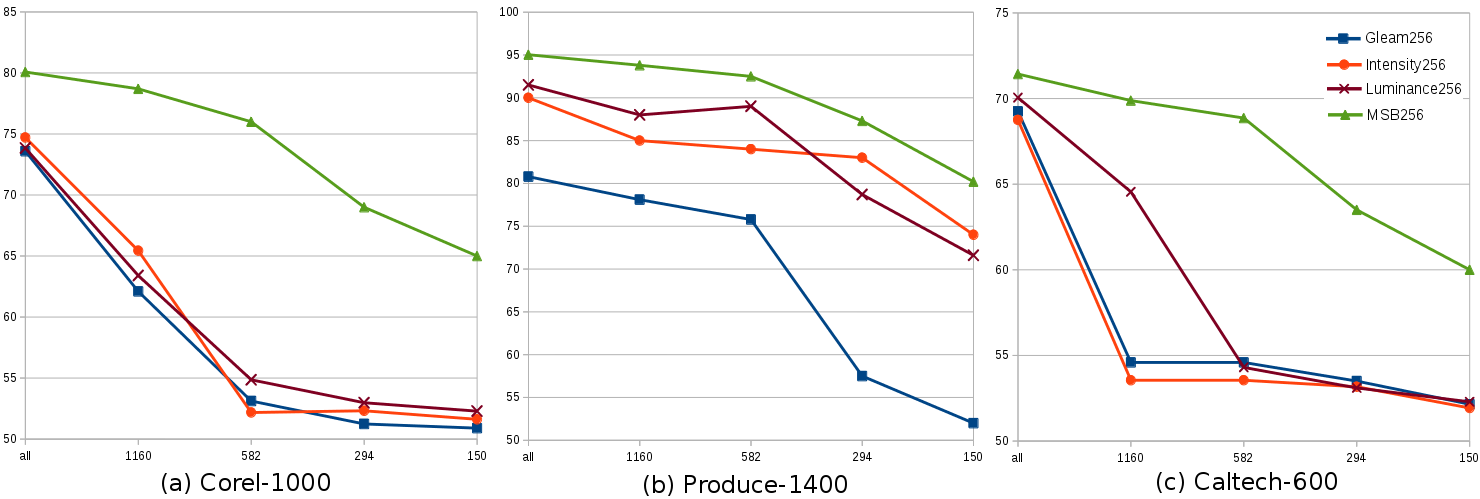
\includegraphics[width=\linewidth]{\detokenize{figuras/quantizacao/fig_results_full.png}}
  \end{center}
  \caption[Comparação da acurácia alcançada com diferentes métodos de quantização: \emph{Gleam}, \emph{Intensidade'}, \emph{Luminância'} e MSB. Inicialmente as imagens foram convertidas para escala de cinza com esses quatro métodos e foram dadas como entrada para todos os métodos de extração. O vetor de características resultante com $D=2310$ sofreu então redução da dimensionalidade com o método LPP para $d = 1160$, $582$, $294$ e $150$.]{Comparação da acurácia alcançada com diferentes métodos de quantização: \emph{Gleam}, \emph{Intensidade'}, \emph{Luminância'} e MSB. Inicialmente as imagens foram convertidas para escala de cinza com esses quatro métodos e foram dadas como entrada para todos os métodos de extração. O vetor de características resultante com $D=2310$ sofreu então redução da dimensionalidade com o método LPP para $d = 1160$, $582$, $294$ e $150$. \\ \textit{Fonte:~\citeonline{Ponti2016}.}}
  \label{fig:quant:resultsFull}
\end{figure}

A utilização de todos os vetores concatenados melhorou a acurácia em relação ao melhor descritor individual. A Figura \ref{fig:quant:resultsFullBoxplot} apresenta a comparação do espaço original com LPP e MSB para redução da dimensionalidade. Os testes estatísticos HSD de Tukey foram realizados utilizando $\alpha = 0.01$ como nível de significância. Os resultados que não mudaram significativamente as acurácias foram: MSB com 582 características para a base de dados \emph{Corel}; e MSB com 1160 para as três bases. O resultado de piora significativa foi para 32 intensidades com a base de imagens Produce-1400. Dados tais resultados, utilizar 64 intensidades é indicado como uma boa escolha do parâmetro de quantização.

\begin{figure}[!htbp]
  \begin{center}
    \centering
    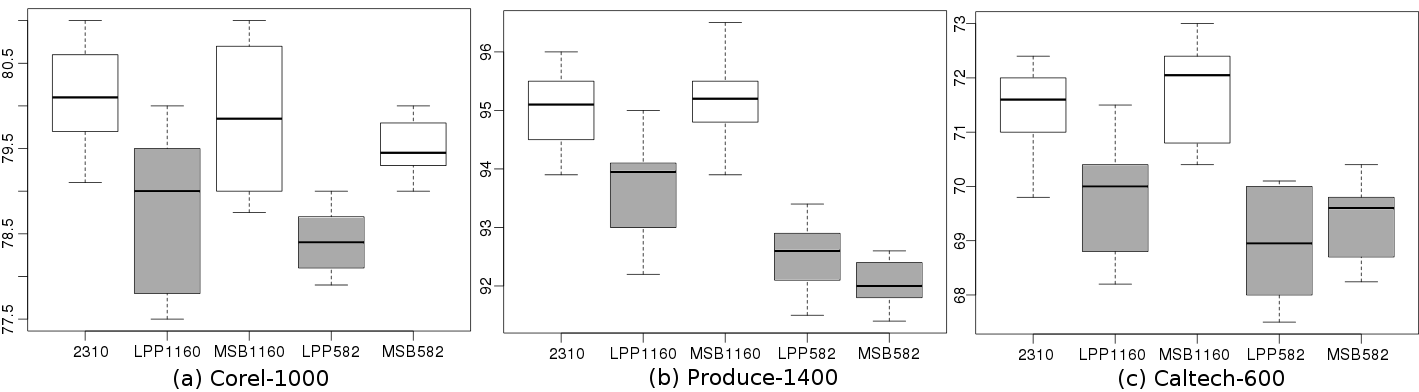
\includegraphics[width=\linewidth]{\detokenize{figuras/quantizacao/fig_results_full_boxplot.png}}
  \end{center}
  \caption[Comparação da acurácia com o uso da projeção LPP e o método MSB para quantização das imagens com o objetivo de redução de dimensionalidade.]{Comparação da acurácia com o uso da projeção LPP e o método MSB para quantização das imagens com o objetivo de redução de dimensionalidade. \\ \textit{Fonte:~\citeonline{Ponti2016}.}}
  \label{fig:quant:resultsFullBoxplot}
\end{figure}

Os resultados indicam que a quantização pode ser utilizada como redução da dimensão de dados visuais, especialmente utilizando 128 e 64 intensidades. Como outro experimento, a Figura~\ref{fig:quant:fullLPP} mostra as acurácias resultantes da aplicação do LPP sob o vetor obtido após a quantização com MSB utilizando 256 e 64 intensidades ($d=2310$ e $d=582$, respectivamente). É interessante notar que as projeções LPP em geral foram melhores com as imagens quantizadas em 64 intensidades com MSB ao invés da original em 256. A razão para isso deve estar no fato da quantização remover informações confusas: ela simplifica as imagens de forma que as intensidades restantes possam melhor descrever uma certa classe.

\begin{figure}[!htbp]
  \begin{center}
    \centering
    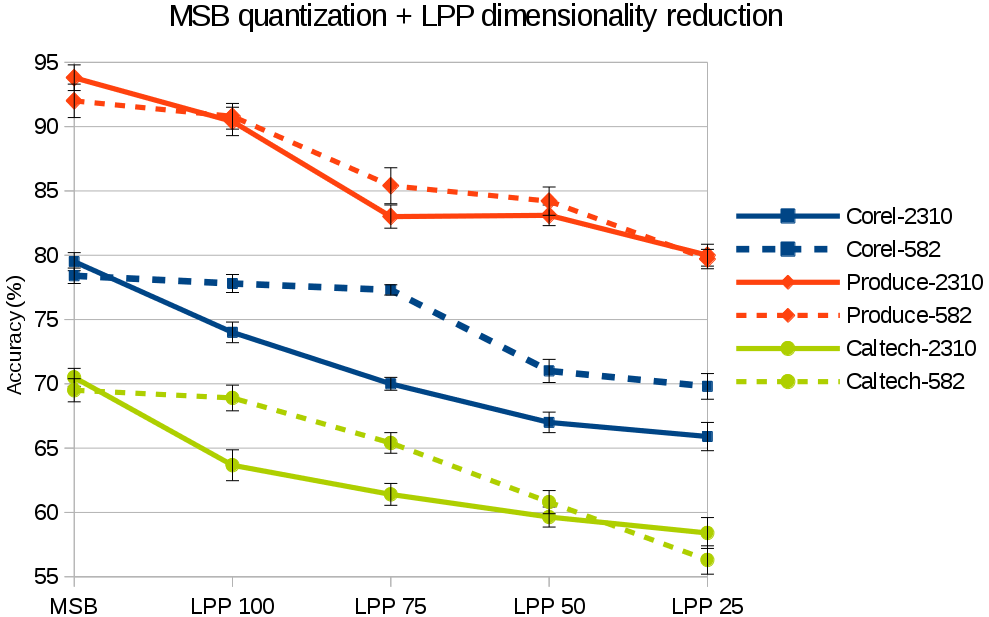
\includegraphics[width=0.6\linewidth]{\detokenize{figuras/quantizacao/fig_results_full_LPP}}
  \end{center}
  \caption[Resultados para a projeção do LPP sobre o espaço de características produzido pelo método de quantização MSB utilizando 256 ($d = 2310$) e 64 intensidades ($d=582$)]{Resultados para a projeção do LPP sobre o espaço de características produzido pelo método de quantização MSB utilizando 256 ($d = 2310$) e 64 intensidades ($d=582$)\\ \textit{Fonte:~\citeonline{Ponti2016}.}}
  \label{fig:quant:fullLPP}
\end{figure}


%%%%%%%%%%%%%%%%%%%%%%%%%%%%%%%%%%%%%%%%%%%%%%%%%%%%%%%%%%%%%%%%%%%%%%%%%%%%%%%%
\section{Considerações finais}

Ao aplicar a quantização na etapa de pré-processamento, obteve-se a redução da dimensionalidade do vetor de características no início do \textit{pipeline}, beneficiando todas as etapas posteriores. Utilizar um número reduzido de intensidades reduziu significativamente a dimensionalidade, enquanto melhorou ou manteve a classificação do sistema. O método MSB para a quantização obteve o melhor desempenho, dada a preservação das intensidades observada na Figura~\ref{fig:quant:avioes}.

Ao comparar o uso da quantização com a utilização de métodos mais complexos para a redução da dimensionalidade, esse processamento permite uma redução significante, enquanto normalmente preserva ou melhora a acurácia do sistema. Independente da utilização de um método de seleção de características, ao escolher um método de quantização apropriado e seus parâmetros é possível reduzir a dimensionalidade e acelerar computacionalmente as etapas que precedem o reconhecimento de imagens. O vetor concatenado com todos os descritores possui $9C + 6$ dimensões, onde $C$ é o número de intensidades da imagem de entrada. O tempo de execução para a extração de todas as características é $f(N) = 42N + 6C^2$, onde $N$ é o número de pixels. Para cada imagem são necessárias $D^2 + kD + d^2$ operações para computar o vetor reduzido com LPP, onde $D$ é o tamanho do vetor original, $d$ o tamanho do vetor de saída e $k$ é o número de vizinhos utilizados no algoritmo. Considere o seguinte exemplo: 100 imagens com 256 intensidades demandam 231.6 milhões de instruções para extrair as características e reduzir o vetor utilizando o método LPP (com $k = 10$ e $d = 50$). Se, ao invés disso, fossem utilizadas 64 intensidades, esse número cairia para 58.7 milhões, o que corresponde a uma redução de 74,6\%.
